\section{Graphs, Cliques, Stable Sets, and Entropy}
\label{tree:poset:graph}

We focus on how to define the information a poset contains. Obviously, in
our decision tree model, a totally ordered set contains maximum information
while a totally unordered set contains no information at all. We have to
understand it this way: If we want to sort a poset, sorting it means acquiring
information on the relation $\le$. If our poset is totally ordered, then we
have all the information needed to describe the relation $\le$ completely. If
the poset contains no information at all, then it means any first $x \ask{\le}
y$ question we might ask gives us exactly $1$ bit of information. In other
words, we cannot deduce any $x \le y$ relation from this poset. Hence, it is
totally unordered.

\subsection{Comparability Graphs}

To help understand the structure of a poset we introduce the comparability
graph ${G}(\P)$\footnote{
Note that, by abuse of notation, we write $G$ to mean ${G}(\P)$.
}
and the incomparability graph $\widetilde{G}(\P)$ of a poset
\(\P\).
\begin{definition}[Comparability graph]
The comparability graph ${G}(\P)$ of a poset $\P$ is an undirected graph whose
vertices are the poset elements, and in which two vertices are adjacent if and
only if the elements are comparable.
\end{definition}
\begin{definition}[Incomparability graph]
The incomparability graph $\widetilde{G}(\P)$ of a poset $\P$ is an undirected
graph whose vertices are the poset elements, and in which two vertices are
adjacent if and only if the elements are incomparable.
\end{definition}

Those graphs explicitly represent all relations (or pairs of incomparable
elements) which may be inferred from the Hasse diagram of $\P$. For example,
the comparability graph of a totally ordered set is the complete graph. See
\ref{fig:comp-graph} for a visual example.



\begin{figure}
\centering
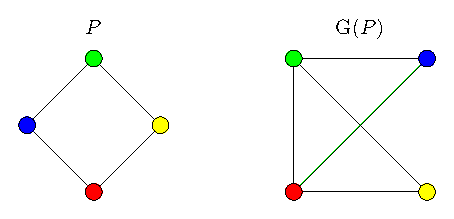
\includegraphics[height=0.15\textheight]{fig/comp-graph}
\caption{\label{fig:comp-graph} A Hasse diagram and its comparability graph.}
\end{figure}




\subsection{Cliques and Stable Sets}

We are interested in analyzing remarkable structures of comparability graphs
like we did before for Hasse diagrams. Indeed, we define hereunder the
counterparts of chains and antichains in posets for comparability graphs.

\begin{definition}[Clique]
A clique $\C$ of graph $G$ is a subset of pairwise adjacent vertices in $G$,
that is, the subgraph induced by $\C$ is complete.
\end{definition}
A clique in a comparability graph ${G}$ is a subset of comparable elements in
$\P$, that is, a chain in $\P$.
A clique in an incomparability graph $\widetilde{G}$ is a subset of
incomparable  elements in $\P$, that is, an antichain in $\P$.

\begin{definition}[Stable set]
A set $\S$ is stable (or independent) if the vertices in $\S$ are pairwise
nonadjacent, that is, the subgraph induced by $\S$ has $\card{\S}$ components.
\end{definition}
A stable set in a comparability graph ${G}$ is a subset of incomparable
elements in $\P$, that is, an antichain in $\P$.
A stable set in an incomparability graph $\widetilde{G}$ is a subset of
comparable elements in $\P$, that is, a chain in $\P$.


A stable set in ${G}$ is a clique in $\widetilde{G}$ and vice versa.



\subsection{$\operatorname{STAB}(G)$}
\label{tree:poset:graph:stab}

In what follows we show that from the internal structure of a graph $G$
expressed using its stable sets we can deduce a discrete distribution
look-alike object. With the help of this object we are able to compute the
entropy of the graph $G$.

We look at our graph $G$ as a ``composition of the
stable sets it contains''. We define $\operatorname{STAB}(G)$ to be the set of convex
combinations of stable sets of $G$.
This set contains all convex combinations (positive,
coefficients summing up to $1$) of characteristic vectors $\chi^{\S}$, where $\S$
is a stable set. The characteristic vector $\chi^{\S}$ is a point in $\R^n$ where
\begin{displaymath}
\chi^{\S}_v =\begin{cases}
      1, & \text{if}\ v \in \S\\
      0, & \text{otherwise}.
    \end{cases}
\end{displaymath}
In other words $\chi^{\S}$ is a binary inclusion/exclusion representation of the
stable set $\S$.
\begin{equation}
\operatorname{STAB}(G) \bydef \operatorname{conv}\enum{\chi^{\S} \in \R^{V(G)} \st
\S\text{ stable set in }G}
\label{eq:stab}
\end{equation}

Formally, \ref{eq:stab} is the definition of the \emph{stable set polytope} of
an arbitrary graph $G$ with vertex set $V(G) = \enum{v_1, \ldots, v_n }$
and order $n$ ($\R^{V(G)} = \R^n, n = \card{V(G)}$) that is, the convex hull (an $n$-dimensional
polytope) of stable set characteristic vectors $\chi^{\S} \in \R^n$.



\subsection{Entropy for Comparability Graphs}

The entropy of a graph can be defined in several ways, see
\citet*{mowshowitz2012entropy} and \citet*{simonyi1995graph}.

Here we define the entropy of a comparability graph $G$ as a function of the
stable sets $G$ possesses. In order to do so, we look at every vector in
$\operatorname{STAB}(G)$ and we keep the vector that gives the lowest entropy
value for a given entropy function. This vector is the discrete distribution
look-alike object we discussed in the previous subsection and the
entropy value is called the entropy of graph $G$, denoted ${H}(G)$.

Formally, we define the entropy of comparability graph $G$ as
\begin{definition}[Entropy of a graph]
\begin{equation}
{H}(G) \bydef \min_{x \in \operatorname{STAB}(G)}~ -\frac{1}{n} \sum_{v \in
V(G)} \log x_v.
\label{eq:entropy:graph}
\end{equation}
\end{definition}

Note that any $x^*$ which minimizes \ref{eq:entropy:graph} also minimizes the
sum on $\log \frac{1}{x_v}$.

The definition of entropy of graphs was first introduced by
\citet*{korner1973coding}. The definition we use is equivalent and is due to
\citet*{csiszar:1990}.


\subsection{Entropy for Posets}

As we defined $H(G)$ in \ref{eq:entropy:graph}, we write $H(\P)$ to mean
$H(G(\P))$. We give a similar definition for \(H(\widetilde{\P})\).
\begin{definition}[Entropy of a poset]
\begin{displaymath}
{H}(\P) \bydef {H}({G}(\P)).
\end{displaymath}
\end{definition}
\begin{definition}[Entropy of the incomparability graph of a poset]
\begin{displaymath}
{H}(\widetilde{\P}) \bydef {H}(\widetilde{G}(\P)).
\end{displaymath}
\end{definition}

Note that since comparability graphs are perfect \cite{berge:1984}, we have
\begin{theorem}[Complementarity of entropies for posets]
For any poset of order \(n\),
\begin{displaymath}
H(\P) + H(\widetilde{\P}) = \log n.
\end{displaymath}
\end{theorem}
